\documentclass{article}
\usepackage{style}
\begin{document}
\maketitle
\tableofcontents
\section{Introducción}
En esta práctica se implementaron los algoritmos:
\begin{itemize}
	\item \textbf{Mutación por Inserción:}
	Se selecciona un valor en forma aleatoria y se le inserta en una posición arbitraria.
	\item \textbf{Mutación por Desplazamiento:} Es una generalizaci´on de la mutaci´on por inserci´on en la que en vez de mover
	un solo valor, se cambian de lugar varios a la vez.
	\item \textbf{Mutación por Intercambio Recíproco:} En este caso, se seleccionan dos puntos al azar y se intercambian estos valores de
	posición.
	\item \textbf{Mutación Heurística:}
	\begin{enumerate}
		\item Seleccionar $\lambda$ genes al azar.
		\item Generar vecinos de acuerdo a todas las permutaciones posibles de los genes
		seleccionados.
		\item Evaluar todos los vecinos y seleccionar el mejor.
	\end{enumerate}
\end{itemize}
\newpage
\section{Contenido}
\subsection{Mutación por Inserción}
\begin{figure}[h!]
	\centering
	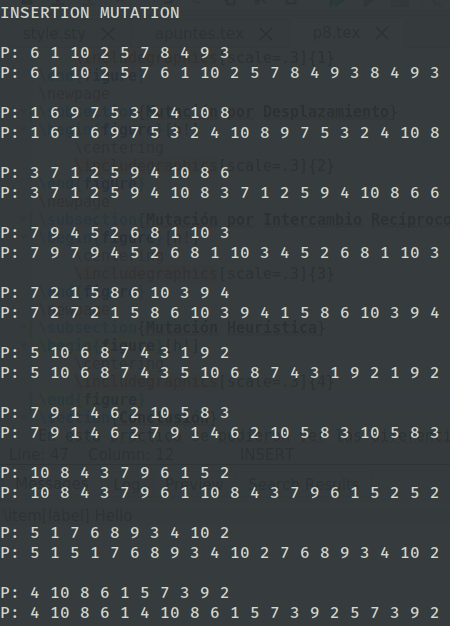
\includegraphics[scale=.3]{1}
\end{figure}
\newpage
\subsection{Mutación por Desplazamiento}
\begin{figure}[h!]
	\centering
	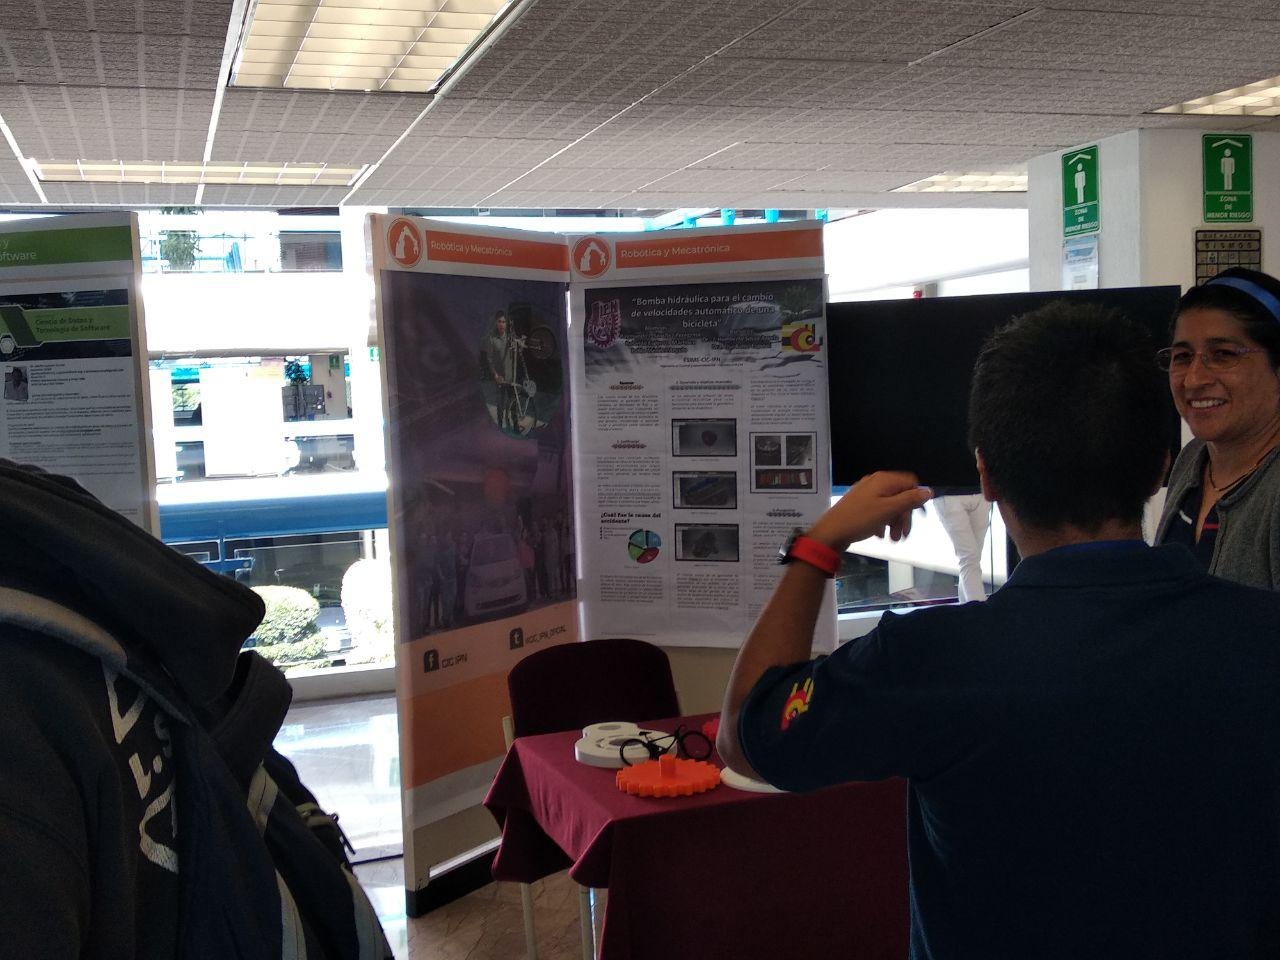
\includegraphics[scale=.3]{2}
\end{figure}
\newpage
\subsection{Mutación por Intercambio Recíproco}
\begin{figure}[h!]
	\centering
	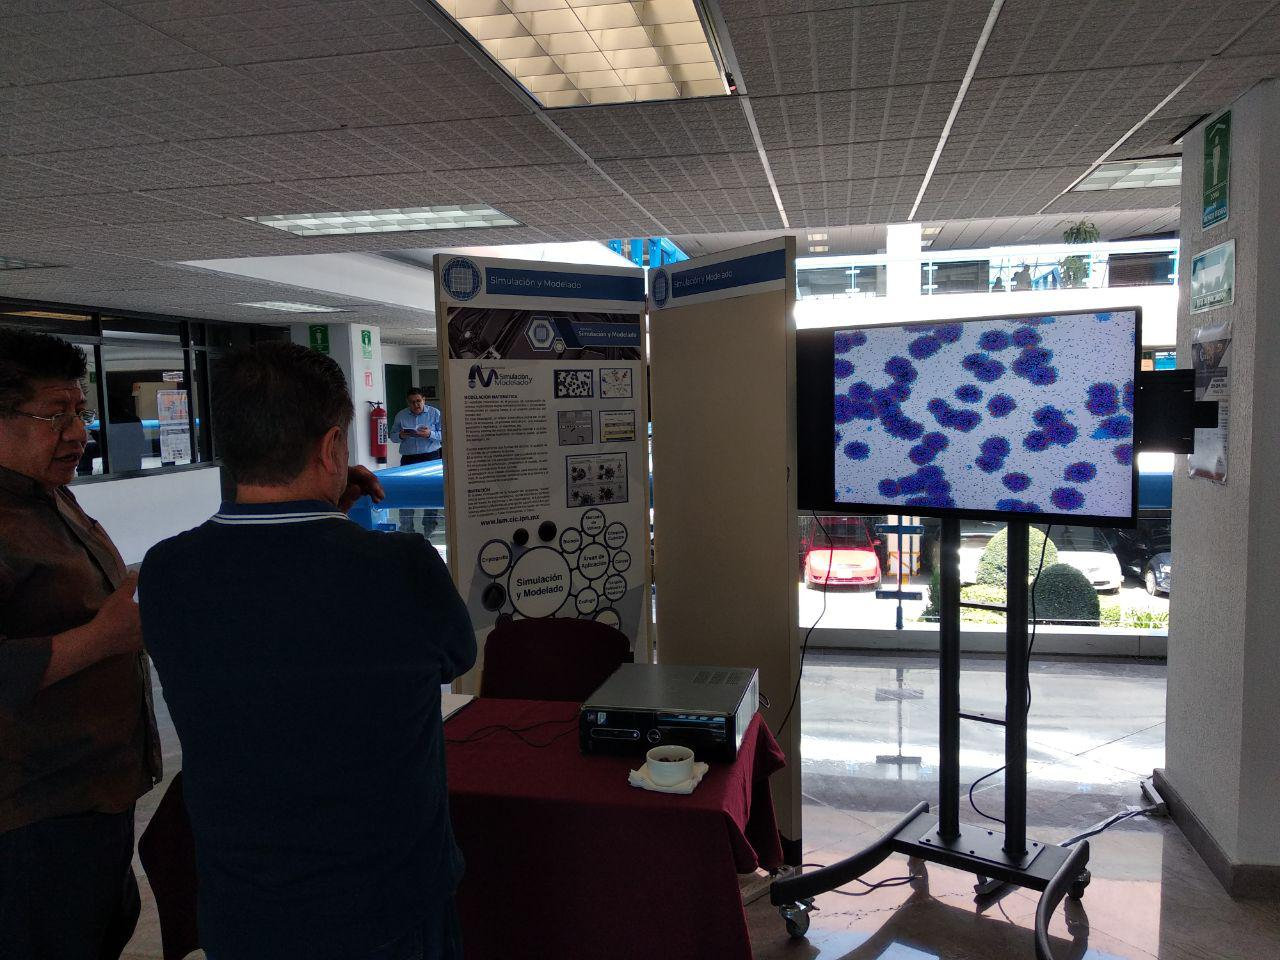
\includegraphics[scale=.3]{3}
\end{figure}
\newpage
\subsection{Mutación Heurística}
\begin{figure}[h!]
	\centering
	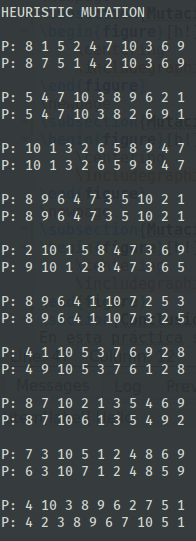
\includegraphics[scale=.3]{4}
\end{figure}
\section{Conclusión}
En esta práctica se pudieron ver las diferencias de algunos de los algoritmos más populares de mutación para permutaciones, se implementaron y se analizaron.
\end{document}